\documentclass{article}

\usepackage{verbatim}
\usepackage{xcolor}
\usepackage{listings}
\usepackage{graphicx}
\usepackage{etoolbox}
\usepackage[most]{tcolorbox}
\usepackage[hidelinks]{hyperref}
\usepackage[nottoc,numbib]{tocbibind}
\hyphenchar\font=-1

\hypersetup{
	allcolors=black
}

\renewcommand{\contentsname}{\'Indice}
\renewcommand\refname{Referencias}

% set the default code style
\lstset{
    language = C,
    frame=tblr, % draw a frame at the top and bottom of the code block
    rulecolor=\color{black},
    tabsize=4, % tab space width
    breakatwhitespace=true,         
    breaklines=true,                 
    captionpos=b,                    
    keepspaces=false,
    showspaces=false,                
    showstringspaces=false,
    showtabs=false,
    basicstyle=\small\ttfamily\bfseries,
    commentstyle=\color{red}, % comment color
    keywordstyle=\color{blue}, % keyword color
    stringstyle=\color{orange} % string color
}
\title{Trabajo Pr\'actico 1: Modelado de Datos}
\date{28-09-2018}
\author{
	Fern\'andez De Luco, Tom\'as\\
	\texttt{F-3443/6}
	\and
	Weinand, Gianni Georg\\
	\texttt{W-0528/2}
	\and
	Molin\'e, Ignacio Sebasti\'an
	\texttt{M-6466/1}
}


\newtcblisting{commandshell}{colback=black,colupper=white,colframe=black,
listing only,listing options={language=sh,  keywordstyle=\color{white}, basicstyle=\small\ttfamily\bfseries, breaklines=true, keepspaces=true, breakatwhitespace=false,  captionpos=b, showstringspaces=false, showtabs=false },
every listing line={\textcolor{pink}{\small\ttfamily\bfseries Monika \$> }}}

\begin{document}

\begin{titlepage}
	\centering
	
\includegraphics[width=0.4\textwidth]{unrlogo}\par\vspace{1cm}
	{\scshape\LARGE R-324 Teor\'ia de Bases de Datos \par}
	\vspace{1cm}
	{\scshape\Large Trabajo Pr\'actico 1\par}
	\vspace{1.5cm}
	{\huge\bfseries Modelado de Datos \par}
	\vspace{2cm}
	{\Large\itshape Tom\'as Fern\'andez de Luco F-3443/6 \\ Gianni Georg Weinand W-0528/2 \\ Ignacio Sebasti\'an Molin\'e M-6466/1 \par}

	\vfill

% Bottom of the page
	{\large 28 de Septiembre, 2018 \par}
\end{titlepage}

\begin{comment}
\tableofcontents

\newpage
\end{comment}

\section{Diagrama Entidad-Relaci\'on}

\begin{align*}
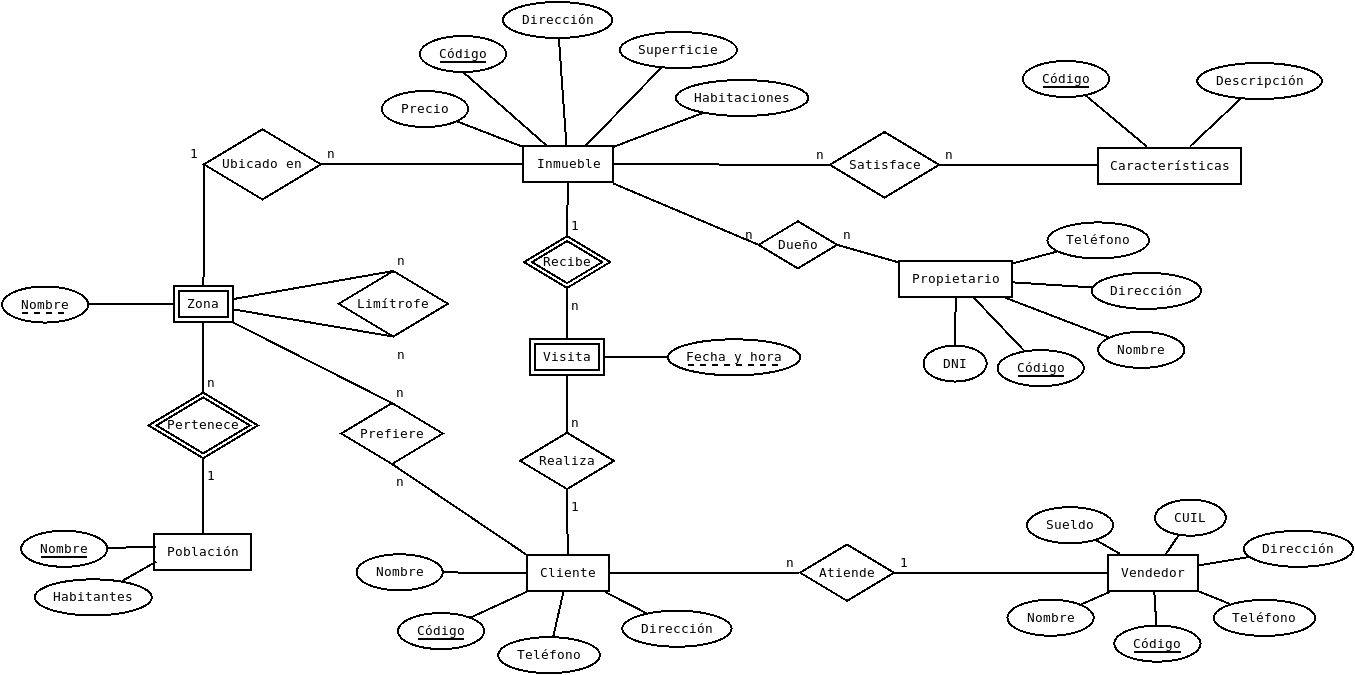
\includegraphics[width=1.2\textwidth, angle = 270]{ER}
\end{align*}

\paragraph{}
Representamos a las visitas como una entidad d\'ebil dependiente de inmueble. La raz\'on de esto es que puede haber un \'unico cliente asignado para visitar por cada combinaci\'on posible de Inmueble y Fecha/Hora. Si la visita hubiera sido una relaci\'on entre Cliente e Inmueble, la clave del Cliente formar\'ia parte de la clave de la Visita y se podr\'ian crear entradas de visitas al mismo Inmueble en la misma Fecha y hora con clientes distintos.

\newpage

\section{Diagrama de Tablas}

\begin{align*}
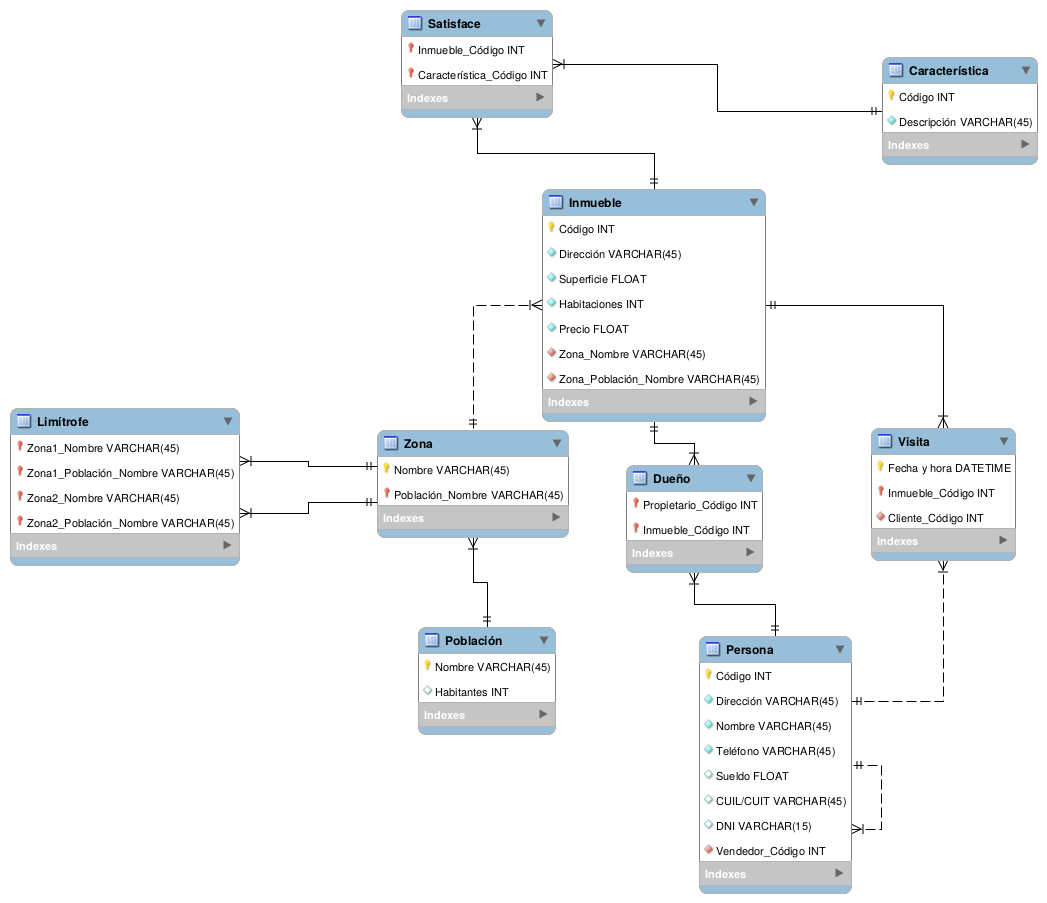
\includegraphics[width=\textwidth]{esq_tablas}
\end{align*}

\paragraph{}
Si bien en el diagrama Entidad-Relaci\'on se consider\'o a los Clientes, Vendedores y Propietarios como entidades separadas sin generalizaci\'on, en el pasaje a tablas se consult\'o la posibilidad de crear una tabla \'unica que tenga algunos campos posiblemente nulos. Como la cantidad de los mismos no era tan grande con respecto al n\'umero de campos en com\'un, se opt\'o por eliminar la redundancia que podr\'ia causarse por tener entradas en varias tablas si una persona cumpliera con m\'as de un rol.
En este caso en particular, suponemos que existir\'ia una cantidad de personas con roles m\'ultiples lo suficientemente relevante como para justificar el incremento en el tamaño de almacenamiento requerido por una entrada en la tabla. Si la redundancia entre categor\'ias fuera baja, ser\'ia recomendable optar por el modelo de tres tablas.

\newpage

\nocite{*}
\bibliography{referencias}
\bibliographystyle{plain}

\end{document}